Veremos el algoritmo de Escaneo de Graham (\emph{Graham's scan}) publicado en 1972 por Graham, y también el algoritmo de Cadena monótona (\emph{Monotone chain}) publicado en 1979 por Andrew.

\subsection{Escaneo de Graham (\emph{Graham's scan})}

El algoritmo primero encuentra el punto más bajo $P_0$. Si hay varios puntos con la misma coordenada Y, se considera el que tiene la coordenada X más pequeña. Este paso toma $O(N)$ tiempo.

A continuación, todos los demás puntos se ordenan por ángulo polar en el sentido de las agujas del reloj. Si el ángulo polar entre dos puntos es el mismo, se elige el punto más cercano.

Luego iteramos a través de cada punto uno por uno, y nos aseguramos de que el punto actual y los dos anteriores hagan un giro en el sentido de las agujas del reloj, de lo contrario, el punto anterior se descarta, ya que tendría una forma no convexa. La verificación de la naturaleza en el sentido de las agujas del reloj o en el sentido contrario a las agujas del reloj se puede realizar comprobando la orientación.

\begin{figure}[!h]
	\centering
	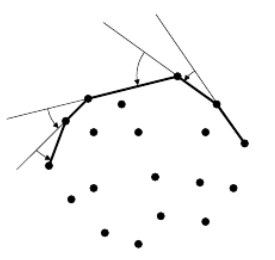
\includegraphics[scale=0.35]{img/cubierta_convexa4}
	\label{fig:cubiertaconvexa2}
\end{figure}

Usamos una pila para almacenar los puntos, y una vez que llegamos al punto original $P_0$, el algoritmo está hecho y devolvemos la pila que contiene todos los puntos del casco convexo en el sentido de las agujas del reloj.

El algoritmo de Graham trabaja de la siguiente forma: 
\begin{itemize}
	\item Sea p$_{i}$  el próximo punto que se agregará al ordenamiento de izquierda a derecha de los puntos.
	\item Si la tripleta { p$_{i}$ , H.first, H.second } tiene orientación positiva, entonces podemos simplemente agregar  p$_{i}$ a la pila
	\item Sino, se puede inferir que le punto medio de la tripleta {\em H.first} no puede estar en la cubierta convexa
	\item Por lo tanto lo borramos de la pila.
	
	\begin{figure}[!h]
		\centering
		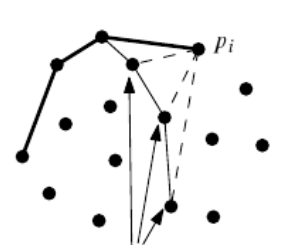
\includegraphics[scale=0.4]{img/cubierta_convexa5}
	\end{figure} 
	\item Ésto es repetido hasta alcanzar una tripleta con orientación positiva, o haya menos de dos elementos en la pila
	
\end{itemize}



Si necesita incluir los puntos colineales mientras realiza un escaneo de Graham, necesita otro paso después de ordenar. Necesita obtener los puntos que tienen la mayor distancia polar de $P_0$ (estos deben estar al final del vector ordenado) y son colineales. Los puntos en esta línea deben invertirse para que podamos generar todos los puntos colineales; de lo contrario, el algoritmo obtendría el punto más cercano en esta línea y saldría. Este paso no debe incluirse en la versión no colineal del algoritmo, de lo contrario no obtendría el casco convexo más pequeño.

\subsection{Cadena monótona (\emph{Monotone chain})}

El algoritmo  es una optimización del algoritmo de Escaneo de Graham (\emph{Graham's scan}) para determinar la cubierta convexa. Este caso se halla de manera separada las cubiertas superior e inferior de la cubierta a continuación una implementación de la misma.

El algoritmo primero encuentra los puntos A y B más a la izquierda y más a la derecha. En el caso de que existan varios puntos de este tipo, el más bajo entre la izquierda (coordenada Y más baja) se toma como A, y el más alto entre la derecha (coordenada Y más alta) es tomado como B. Claramente, A y B deben pertenecer ambos al casco convexo ya que son los más alejados y no pueden ser contenidos por ninguna línea formada por un par entre los puntos dados.

Ahora, dibuja una línea a través de AB. Esto divide todos los demás puntos en dos conjuntos, S1 y S2, donde S1 contiene todos los puntos por encima de la línea que une A y B, y S2 contiene todos los puntos por debajo de la línea que une A y B. Los puntos que se encuentran en la línea que une A y B pueden pertenecer a cualquiera de los conjuntos. Los puntos A y B pertenecen a ambos conjuntos. Ahora el algoritmo construye el conjunto superior S1 y el conjunto inferior S2 y luego los combina para obtener la respuesta.

Para obtener el conjunto superior, ordenamos todos los puntos por la coordenada x. Para cada punto, verificamos si el punto actual es el último punto (que definimos como B), o si la orientación entre la línea entre A y el punto actual y la línea entre el punto actual y B es en el sentido de las agujas del reloj. En esos casos el punto actual pertenece al conjunto superior S1. La verificación de la naturaleza en el sentido de las agujas del reloj o en el sentido contrario a las agujas del reloj se puede realizar comprobando la orientación.

Si el punto dado pertenece al conjunto superior, comprobamos el ángulo formado por la línea que une el penúltimo punto y el último punto del casco convexo superior, con la línea que une el último punto del casco convexo superior y el punto actual. Si el ángulo no es en el sentido de las agujas del reloj, eliminamos el punto más reciente agregado al casco convexo superior ya que el punto actual podrá contener el punto anterior una vez que se agregue al casco convexo.

La misma lógica se aplica para el conjunto inferior S2. Si el punto actual es B, o la orientación de las líneas, formadas por A y el punto actual y el punto actual y B, es en sentido contrario a las agujas del reloj, entonces pertenece a S2.

Si el punto dado pertenece al conjunto inferior, actuamos de manera similar a un punto en el conjunto superior excepto que verificamos una orientación en sentido contrario a las manecillas del reloj en lugar de una orientación en el sentido de las manecillas del reloj. Por lo tanto, si el ángulo formado por la línea que conecta el penúltimo punto y el último punto en el casco convexo inferior, con la línea que conecta el último punto en el casco convexo inferior y el punto actual no es en sentido antihorario, eliminamos el punto más reciente agregado al casco convexo inferior como el punto actual podrá contener el punto anterior una vez agregado al casco.

El casco convexo final se obtiene de la unión del casco convexo superior e inferior, formando un casco en el sentido de las agujas del reloj, y la realización es la siguiente.

Si necesita puntos colineales, solo necesita buscarlos en las rutinas en sentido horario/antihorario. Sin embargo, esto permite un caso degenerado en el que todos los puntos de entrada son colineales en una sola línea y el algoritmo generaría puntos repetidos. Para resolver esto, verificamos si el casco superior contiene todos los puntos, y si los contiene, simplemente devolvemos los puntos al revés, ya que eso es lo que devolvería la implementación de Graham en este caso.
